\documentclass[crop,tikz]{standalone}
\usepackage{tikz}
\usepackage{graphicx}
\usetikzlibrary{shapes.geometric,arrows, fit}
\usepackage{adjustbox}
\usetikzlibrary{decorations.pathreplacing}
\usepackage{float}
\usetikzlibrary{matrix,backgrounds,positioning}
\usetikzlibrary{shadows}
\usetikzlibrary{decorations.pathmorphing}
\usetikzlibrary{arrows, decorations.markings}
\usetikzlibrary{arrows.meta,calc}
\usepackage{xcolor}



\definecolor{amethyst}{rgb}{0.6, 0.4, 0.8}
\definecolor{asparagus}{rgb}{0.53, 0.66, 0.42}
\definecolor{airforceblue}{rgb}{0.36, 0.54, 0.66}
\definecolor{brightlavender}{rgb}{0.75, 0.58, 0.89}
\definecolor{MyBlue}{rgb}{0.25,0.5,0.75}
\definecolor{arylideyellow}{rgb}{0.91, 0.84, 0.42}



\begin{document}
\begin{tikzpicture}
	         \tikzset{
        model/.style= {draw, rectangle, align=center,text width=2 cm,minimum height=1 cm, fill=yellow!30},
          cube join/.style={
    thick, -{Stealth}, 
  },
  cube face/.style={
    minimum size=1.2cm, outer sep=0pt,
    draw=gray, line join=round,
    text=white, font=\bfseries
  },    
  pics/cube/.style args={#1 with #2}{
  code={
    \node [cube face, fill=cyan!40] (-front) {};
    \node [cube face, fill=cyan!20] (-top)  at (-front.north west) [anchor=south west, xslant=1, yscale=1/3] {};
    \node [cube face, fill=cyan!60] (-side) at (-front.south east) [anchor=south west, yslant=1, xscale=1/3] {};
   }},
      cascaded/.style = {%
    general shadow = {%
      shadow scale = 1,
      shadow xshift = 2ex,
      shadow yshift = 2ex,
      draw=black,
      fill = asparagus!20},
    general shadow = {%
      shadow scale = 1,
      shadow xshift = 1.5ex,
      shadow yshift = 1.5ex,
      draw=black,
      fill = asparagus!20},
    general shadow = {%
      shadow scale = 1,
      shadow xshift = 1ex,
      shadow yshift = 1ex,
      draw=black,
      fill = asparagus!20},
    general shadow = {%
      shadow scale = 1,
      shadow xshift = .5ex,
      shadow yshift = .5ex,
      draw=black,
      fill = asparagus!20},
    fill = asparagus!20, 
    draw},
subblock/.style= {draw, rectangle,rounded corners=0.3em, align=center,minimum width=0.55cm,minimum height=0.2cm, fill=brightlavender},
cube1 face/.style={
    minimum size=0.6cm, outer sep=0pt,
    draw=gray, line join=round,
    text=white, font=\bfseries
  },    
  pics/cube1/.style args={#1 with #2}{
  code={
    \node [cube1 face, fill=airforceblue!40] (-front) {};
    \node [cube1 face, fill=airforceblue!20] (-top)  at (-front.north west) [anchor=south west, xslant=1, yscale=1/5] {};
    \node [cube1 face, fill=airforceblue!60] (-side) at (-front.south east) [anchor=south west, yslant=1, xscale=1/5] {};
   }}
    }
    
    \node(main) at (0,0){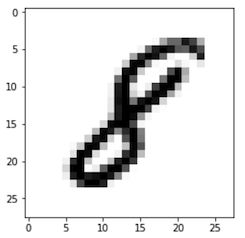
\includegraphics[width=.3\textwidth]{digit.png}};
    
\node(fasta)[right of=main, node distance = 4.5 cm]{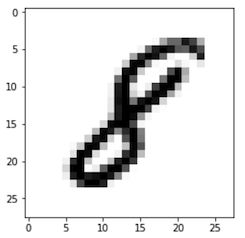
\includegraphics[width=.3\textwidth]{digit.png}};
\draw[red,ultra thick] ($(fasta.south west) + (2.5,2.5)$) rectangle ($(fasta.south west) + (3.4,3.4)$);


%\node[anchor=south west,inner sep=0] (image)


\node [cascaded, fill = arylideyellow!60,  minimum width = 5em, minimum height = 5em, right= of fasta, node distance = 0.1 cm] (conv1) {};

\draw[fill= amethyst] ($(conv1.south west) + (0.3,0.3)$) rectangle ($(conv1.south west) + (0.6,0.6)$);

\node [cascaded, fill = arylideyellow!60,  minimum width = 5em, minimum height = 5em, right= of conv1, node distance = 0.1 cm] (conv2) {};

\draw[fill= amethyst] ($(conv2.south west) + (0.3,0.3)$) rectangle ($(conv2.south west) + (0.6,0.6)$);

\node [cascaded, fill = arylideyellow!60,  minimum width = 5em, minimum height = 5em, right= of conv2, node distance = 0.1 cm] (conv3) {};

\draw[fill= amethyst] ($(conv3.south west) + (0.3,0.3)$) rectangle ($(conv3.south west) + (0.6,0.6)$);


\pic [local bounding box=A1, right of = conv3, node distance = 3.8 cm, yshift = 0.5 cm]  {cube=1 with $C$};
\pic [local bounding box=A2, left of=A1, node distance=0.8 cm, yshift =-0.8 cm]{cube=1 with $C$};
\pic [local bounding box=A3, left of=A2, node distance=0.8 cm, yshift =-0.8 cm]{cube=1 with $C$};

\pic [local bounding box=A4, below of=conv1, node distance=0.1 cm, yshift =0.2 cm,xshift= 0.25cm]{cube1=1 with $C$};
\pic [local bounding box=A5, below of=conv2, node distance=0.1 cm, yshift =0.2 cm,xshift= 0.25cm]{cube1=1 with $C$};
\pic [local bounding box=A6, below of=conv3, node distance=0.1 cm, yshift =0.2 cm,xshift= 0.25cm]{cube1=1 with $C$};

\draw[fill= amethyst] ($(A3.south west) + (0.3,0.3)$) rectangle ($(A3.south west) + (0.6,0.6)$);

  \matrix (digi_cap) [right=1.5 cm of A2, matrix of nodes,minimum width=1cm, minimum height=0.7cm, row sep=-\pgflinewidth, nodes={draw=white, fill=gray!90}]
	{
		{}  \\
		{}  \\
        {} \\
		{}  \\
        {}  \\
        {}  \\
        {}  \\
	};   

\node [subblock,right of=digi_cap, node distance=1.8 cm] (cp1) {};
\node [subblock,right of=cp1, node distance=0.7 cm] (cp2) {};
\node [right of=cp2, node distance=0.6 cm] (d1) {$\dots$};
\node [subblock,right of=d1, node distance=0.7 cm] (cp3) {};

\node[fit= (cp1) (cp3), fill= gray,draw, opacity= 0.4, inner sep=0.1cm, rounded corners] (box){};


\foreach \l [count=\i] in {1,...,3}
    \draw[decorate,thick, decoration={brace, amplitude=8pt}] ($(conv\i)+(1.5, -1.05)$) -- coordinate [above=0pt] (mid\i)++ (-2.5,0) node {};



\node[below of = main, align = center, node distance = 2 cm] () {Input Picture};
\node[below of = mid1, align = center, node distance = 0.7 cm] () {ReLU Conv1};
\node[below of = mid2, align = center, node distance = 0.7 cm] () {ReLU Conv2};
\node[below of = mid3, align = center, node distance = 0.7 cm] () {ReLU Conv3};
\node[fit= {(A1)(A3)($(A2.south)+(0,-1.1)$)},line width=0.5mm, draw, dashed,inner sep=0.3cm] (PB){};
\node[below of = PB, align = center, node distance=2.3 cm] () {\Large{Primary Caps}};
\node [below of=digi_cap, node distance=2.9 cm] () {\large{Secondary Caps}};
\node [below of=box, node distance=0.8 cm] () {\large{Class capsules}};


\draw[dashed, thick] ($(fasta.south west) + (3.4,3.4)$) -- ($(conv1.south west) + (0.3,0.6)$);
\draw[dashed, thick] ($(fasta.south west) + (3.4,2.5)$) -- ($(conv1.south west) + (0.3,0.3)$);
\draw[dashed, thick] (A4.north east) -- ($(conv2.south west) + (0.3,0.6)$);
\draw[dashed, thick](A4.south east) -- ($(conv2.south west) + (0.3,0.3)$);
\draw[ dashed, thick] (A5.north east) -- ($(conv3.south west) + (0.3,0.6)$);
\draw[dashed, thick](A5.south east) -- ($(conv3.south west) + (0.3,0.3)$);
\draw[dashed, thick] (A6.north east) -- ($(A3.south west) + (0.3,0.6)$);
\draw[dashed, thick](A6.south east) -- ($(A3.south west) + (0.3,0.3)$);
\draw[dashed, thick](A1.north east) -- (digi_cap-1-1.north west);
\draw[dashed, thick]($(A3.south east)+(-0.5,0)$) -- (digi_cap-7-1.south west);
\draw[>={LaTeX[width=6mm,length=3mm]},->, MyBlue, line width=3mm] (main) -- (fasta);
\draw[>={LaTeX[width=6mm,length=3mm]},->, MyBlue, line width=3mm] (digi_cap) -- (box);

\end{tikzpicture}
\end{document}